\section{弱对偶}
\label{sec:dual-weak}

上一节在例子里反复看到“下界不超过最优值”。这个结论在什么范围内成立，它又能为手里的候选点提供什么？

\begin{theorem}[弱对偶]
 \label{thm:dual-weak}
 对问题~\eqref{eq:dual-primal}的任一可行点$\bm{x}$和任一组$\bm{\lambda}\geq\bm{0}$、$\bm{\nu}$，有
 \begin{equation}
  q(\bm{\lambda},\bm{\nu})\leq f(\bm{x}).
  \label{eq:dual-weak-pair}
 \end{equation}
 因而
 \begin{equation}
  d^\star\leq f^\star.
  \label{eq:dual-weak}
 \end{equation}
\end{theorem}

\begin{proof}
 由可行性和$\bm{\lambda}\geq\bm{0}$，有$\lambda_ig_i(\bm{x})\leq0$和$\nu_jh_j(\bm{x})=0$，所以这些项都不使$f(\bm{x})$增大。又因为$\bm{x}\in\bm{D}$，由下确界的定义，
 \[
  q(\bm{\lambda},\bm{\nu})\leq\mathcal{L}(\bm{x},\bm{\lambda},\bm{\nu})\leq f(\bm{x}).
 \]
 左边不含$\bm{x}$，对可行点取下确界，再对合法乘子取上确界，就得到式~\eqref{eq:dual-weak}。没有可行点时$f^\star=+\infty$，式~\eqref{eq:dual-weak}自然成立。
\end{proof}

证明只用了两件事：下确界的定义，以及符号。它不需要凸性，不需要可微性，也不需要任何约束资格。正因为条件这样少，弱对偶可以用于任何问题，这是它最大的价值。

\term{弱对偶}这个名字在第~\ref{chap:linear-programming}章已经出现过，那里说的是线性规划的特例。两个差要分清。一个是某一对候选的差$f(\bm{x})-q(\bm{\lambda},\bm{\nu})$，下面称为\emph{候选间隙}，算法每一步都能算出。另一个是两个最优值的差$f^\star-d^\star$，这是问题本身的性质，称为\term{对偶间隙}。候选间隙总不小于对偶间隙。

\paragraph{在目标—约束平面上看弱对偶}
把每个$x$映成平面上的一点$(u,t)=(g(x),f(x))$，横坐标是约束值，纵坐标是目标值，这些点组成集合$\bm{G}$。对一元例，$u=x-1$，$t=\frac12(u-1)^2$，$\bm{G}$是一条抛物线，如图~\ref{fig:dual-image-set}所示。可行点对应$u\leq0$，原始问题就是在竖线左侧找$\bm{G}$的最低点。

$\mathcal{L}=t+\lambda u$在斜率为$-\lambda$的直线上为常数。$q(\lambda)$就是把这样的直线从下方推到刚好碰到$\bm{G}$，这条直线与竖轴$u=0$的交点高度。

所以弱对偶的几何含义是：直线在$\bm{G}$下方，$\lambda\geq0$时它在$u\leq0$一侧向左不下降，因此$\bm{G}$中$u\leq0$的部分都在交点上方。对偶问题就是转动直线，使交点尽量高。$\lambda$取负数时直线向左下降，交点就可能高过可行部分的最低点，后面会看到这个现象。

\begin{BookInlineFigure}
 \centering
 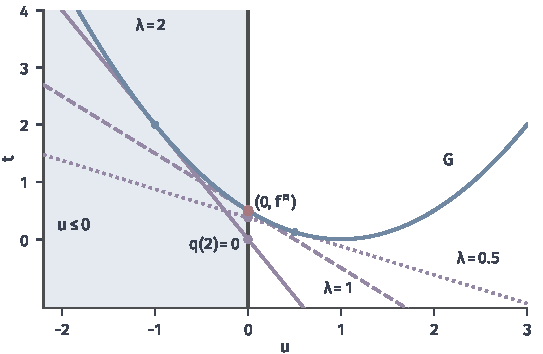
\includegraphics[width=92mm]{figures/05-optimization/06-constrained-optimization/matplotlib/dual-image-set/figure.pdf}
 \caption{一元例在$(u,t)=(g(x),f(x))$平面上的像。蓝线是$\bm{G}$，浅蓝区域是可行的半平面$u\leq0$，深灰粗线是$u=0$。紫线是斜率$-\lambda$的支撑直线（$\lambda=0.5,1,2$，分别为点线、虚线、实线），它们在$\bm{G}$下方，与$u=0$的交点（紫点）高度就是$q(\lambda)$，分别为$0.375$、$0.5$、$0$。红点$(0,f^\star)$是$\lambda=1$时的切点。}
 \label{fig:dual-image-set}
\end{BookInlineFigure}

\subsection{可行候选的误差证书}
\label{sec:dual-certificate}

现在回答本章开头的问题。手里有一个可行点$\hat{\bm{x}}$和一组合法乘子$(\bm{\lambda},\bm{\nu})$，由弱对偶，最优值被夹在两个可计算的数之间：
\begin{equation}
 q(\bm{\lambda},\bm{\nu})\leq f^\star\leq f(\hat{\bm{x}}).
 \label{eq:dual-sandwich}
\end{equation}
两边同时减去，得到次优性的一个可以计算的上界：
\begin{equation}
 0\leq f(\hat{\bm{x}})-f^\star\leq f(\hat{\bm{x}})-q(\bm{\lambda},\bm{\nu}).
 \label{eq:dual-gap-certificate}
\end{equation}
右端不含$f^\star$，这一对候选本身就是一份\emph{误差证书}。第~\ref{chap:optimization}章讨论过目标差难以计算的困难，这里给出了一种解决办法。

用二次例算一组不是最优的候选。取可行点和乘子
\[
 \hat{\bm{x}}=\Bigl(\frac34,\frac14\Bigr),\qquad\nu=-\frac34.
\]
原始目标值由定义计算，对偶目标值由式~\eqref{eq:dual-quad-q}计算：
\[
 f(\hat{\bm{x}})=\frac12\Bigl(\frac{9}{16}+\frac{4}{16}\Bigr)=\frac{13}{32},\qquad
 q\Bigl(-\frac34\Bigr)=-\frac{45}{128}+\frac34=\frac{51}{128}.
\]

候选间隙是
\[
 \frac{13}{32}-\frac{51}{128}=\frac{52-51}{128}=\frac{1}{128}\approx0.0078.
\]
所以不用知道答案，我们就确认$\hat{\bm{x}}$的目标差不超过$0.0078$。

因为这个例子知道答案，可以核对证书有多紧。真实目标差和乘子一侧的差分别是
\[
 \frac{13}{32}-\frac25=\frac{1}{160},\qquad\frac25-\frac{51}{128}=\frac{1}{640}.
\]
两者之和是
\[
 \frac{1}{160}+\frac{1}{640}=\frac{5}{640}=\frac{1}{128},
\]
正是候选间隙。候选间隙同时度量了原始和对偶两侧的误差，图~\ref{fig:dual-certificate-line}把这几个数放在同一条数轴上。

\begin{BookInlineFigure}
 \centering
 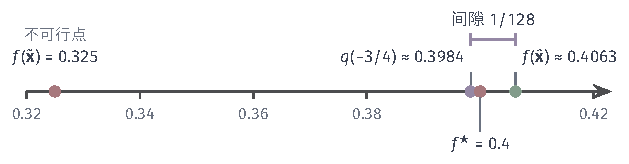
\includegraphics[width=106.4mm]{figures/05-optimization/06-constrained-optimization/tikz/dual-certificate-line/figure.pdf}
 \caption{二次例的误差证书。紫点是下界$q(-3/4)$，绿点是可行点$\hat{\bm{x}}$的目标值，红点$f^\star$夹在两者之间，紫色括线是候选间隙。左边的红点是不可行点$\tilde{\bm{x}}=(0.7,0.2)$的目标值，它比$f^\star$低，不能用来估计误差。}
 \label{fig:dual-certificate-line}
\end{BookInlineFigure}

式~\eqref{eq:dual-gap-certificate}有三个前提，每一个都要单独检验，下面逐一看缺了会怎样。

第一个是原始可行性。点$\tilde{\bm{x}}=(0.7,0.2)$不满足约束，因为$0.7+0.2\neq1$。它的目标值只有
\[
 f(\tilde{\bm{x}})=\frac12(0.49+0.16)=0.325,
\]
比最优值低，与下界的差是$0.325-0.3984\approx-0.073$，是负数。负的“间隙”在这里暴露了不可行，但一般不能指望这样：不可行点也可能给出正的小间隙。所以约束残差要另外计算，不能从间隙看出来。

第二个是乘子的合法性。考虑$\min x^2$，约束$x-1\leq0$，最优值$f^\star=0$。内层最小点是$x=-\lambda/2$，代回得到
\[
 q(\lambda)=-\frac{\lambda^2}{4}-\lambda.
\]
这个公式对负的$\lambda$照样能算，例如$\lambda=-2$时给出$q=1$，比真实最优值$0$还大。

错在哪里？$\lambda=-2$时，可行点$x=0$上的$\mathcal{L}=0-2(0-1)=2$，比$f(0)=0$大，证明中$\mathcal{L}\leq f$这一步失效。图~\ref{fig:dual-illegal-multiplier}中红色虚线高过了$f^\star$，这段就是不合法的乘子。

\begin{BookInlineFigure}
 \centering
 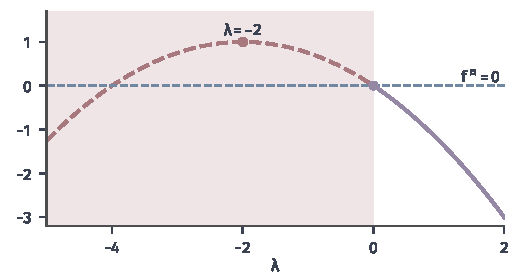
\includegraphics[width=88mm]{figures/05-optimization/06-constrained-optimization/matplotlib/dual-illegal-multiplier/figure.pdf}
 \caption{乘子合法性的作用。问题是$\min x^2$，约束$x-1\leq0$。紫线是$\lambda\geq0$时的$q(\lambda)$，始终不超过蓝色虚线$f^\star=0$；红色虚线和浅红区域对应$\lambda<0$，同一个公式在这里可以超过$f^\star$，例如$\lambda=-2$时为$1$，它不是下界。}
 \label{fig:dual-illegal-multiplier}
\end{BookInlineFigure}

第三个前提是下界本身算得可信，也就是内层下确界确实是下确界。这一点在实际计算中最容易被忽略，单独放在下一小节讨论。

\subsection{内层近似的方向}
\label{sec:dual-inexact-inner}

计算$q$需要解一个最小化问题。多数情况下内层得不到解析解，只能迭代到某个近似点$\tilde{\bm{x}}$。这样算出的$\mathcal{L}(\tilde{\bm{x}},\bm{\lambda},\bm{\nu})$可不可以当作下界使用？

答案是不可以，而且误差的方向恰好不对。由下确界的定义，
\[
 \mathcal{L}(\tilde{\bm{x}},\bm{\lambda},\bm{\nu})\geq q(\bm{\lambda},\bm{\nu}),
\]
近似值落在真正下界的\emph{上方}。普通的数值误差只让答案不够精确，这里的误差却可能让“下界”超过最优值，于是证书本身失效。

还是看二次例，固定$\nu=-3/4$。精确的内层解是$\bm{x}(\nu)=(3/4,3/16)$。假设迭代停在
\[
 \tilde{\bm{x}}=(0.8,0.15).
\]
此处的Lagrange函数值是
\[
 \mathcal{L}(\tilde{\bm{x}},\nu)=\frac12(0.64+0.09)-0.75\,(0.8+0.15-1)=0.365+0.0375=0.4025.
\]
这个数比$f^\star=0.4$还大。如果把它当作下界，就会得出一个错误的结论，以为最优值不小于$0.4025$。

要得到可靠的下界，必须从近似值中扣除一个经过证明的量。若内层函数有已知的曲率下界，用梯度残差就可以写出这个量。

\begin{lemma}[由梯度残差得到的认证下界]
 \label{lem:dual-certified-bound}
 设$\bm{D}=\mathbb{R}^n$，$\bm{\lambda}\geq\bm{0}$，函数$\mathcal{L}(\cdot,\bm{\lambda},\bm{\nu})$可微且是$\mu$强凸的，$\mu>0$。则对任意$\tilde{\bm{x}}$，
 \begin{equation}
  q(\bm{\lambda},\bm{\nu})\geq\mathcal{L}(\tilde{\bm{x}},\bm{\lambda},\bm{\nu})-\frac{1}{2\mu}\bigl\lVert\nabla_{\bm{x}}\mathcal{L}(\tilde{\bm{x}},\bm{\lambda},\bm{\nu})\bigr\rVert_2^2.
  \label{eq:dual-certified-bound}
 \end{equation}
\end{lemma}

\begin{proof}
 记$\phi=\mathcal{L}(\cdot,\bm{\lambda},\bm{\nu})$，$\bm{r}=\nabla\phi(\tilde{\bm{x}})$。由$\mu$强凸的一阶不等式，对任意$\bm{y}$，
 \[
  \phi(\bm{y})\geq\phi(\tilde{\bm{x}})+\langle\bm{r},\bm{y}-\tilde{\bm{x}}\rangle+\frac{\mu}{2}\lVert\bm{y}-\tilde{\bm{x}}\rVert_2^2.
 \]
 右端是$\bm{y}$的二次函数，在$\bm{y}=\tilde{\bm{x}}-\bm{r}/\mu$处最小，最小值为$\phi(\tilde{\bm{x}})-\lVert\bm{r}\rVert_2^2/(2\mu)$。于是对任意$\bm{y}$，
 \[
  \phi(\bm{y})\geq\phi(\tilde{\bm{x}})-\frac{1}{2\mu}\lVert\bm{r}\rVert_2^2.
 \]
 对$\bm{y}$取下确界即得。
\end{proof}

式~\eqref{eq:dual-certified-bound}的含义是：曲率下界$\mu$限制了函数在$\tilde{\bm{x}}$附近能下降多少，碗不会比它更平，所以梯度残差所能带来的下降有上限，我们把这个上限全部扣掉。

代入例子。Hessian是$\operatorname{diag}(1,4)$，取$\mu=1$。梯度和扣除量分别是
\[
 \nabla_{\bm{x}}\mathcal{L}(\tilde{\bm{x}},\nu)=(x_1+\nu,\,4x_2+\nu)=(0.05,-0.15),\qquad\frac{1}{2\mu}\lVert\cdot\rVert_2^2=\frac{0.025}{2}=0.0125.
\]
认证下界是
\[
 0.4025-0.0125=0.39.
\]

它确实低于真正的$q(-3/4)=0.3984$。图~\ref{fig:dual-inner-approx}把这些数排在一起：未修正的内层值在$f^\star$上方，认证下界在$q$下方。把它和$f(\hat{\bm{x}})=0.40625$配对，得到的候选间隙是$0.01625$，比精确内层的$0.0078$宽，但它是可信的。

\begin{BookInlineFigure}
 \centering
 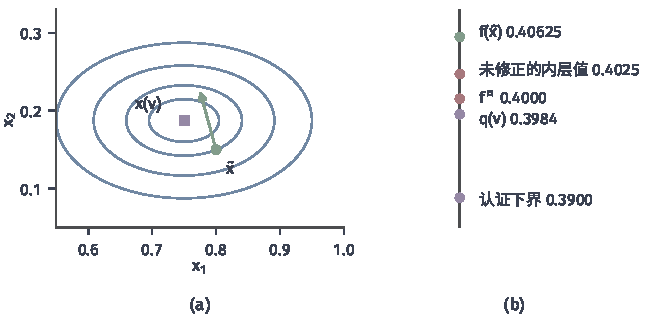
\includegraphics[width=112mm]{figures/05-optimization/06-constrained-optimization/matplotlib/dual-inner-approx/figure.pdf}
 \caption{近似内层的方向。(a)~蓝线是$\mathcal{L}(\cdot,-3/4)$的等高线，紫色方块是精确内层解$\bm{x}(\nu)$，绿点是近似点$\tilde{\bm{x}}$，绿色箭头是负梯度方向。(b)~数轴上由下往上是认证下界、精确的$q(\nu)$、$f^\star$、未修正的内层值和可行点的目标值；未修正的内层值高于$f^\star$，不能当作下界。}
 \label{fig:dual-inner-approx}
\end{BookInlineFigure}

式中的$\mu$必须是真正的曲率下界。若误把$\mathcal{L}$的最大曲率$4$当作$\mu$，扣除量只有$0.025/8=0.003125$，得到$0.399375$，已经超过真正的$q=0.3984$，证书不再成立。当内层没有已知的强凸常数，或者$\bm{D}$不是全空间时，这个引理不能直接使用；此时内层的近似值只能算是一个估计，不能写进误差证书。
